\appendix{Websockets vs. TCP speed}

Websocket is an HTML5 standard aiming at overcoming all the shortcomings of the
already-old HTTP protocol in real-time client-server communication. It is a
TCP-based protocol that uses an HTTP handshake - but that's where the
commonalities stop. The main issue that WS(Websockets) addresses is that with
HTTP, a server cannot send information to the client without being solicited.
Also, WS connections can be kept open and thus bidirectional communication can
be kept alive.\newline

A thorough search for benchmarks for the latency of Websockets versus raw TCP
has returned no result. Instead, several have been found of comparisons between
Websockets and HTTP, Comet and Ajax. Interesting information is found on the
Websocket.org website and reproduced here: \newline

Figure \ref{fig:websocket_frame} shows the size overhead of a Websocket frame
over raw TCP is 2bytes. Figure \ref{fig:websocket_ws_vs_polling} shows the
overhead(in bits per second) of HTTP Polling versus Websockets. We can notice
that in both cases the scale is linear, but the factor is much smaller for
Websockets.\newline

\begin{figure}
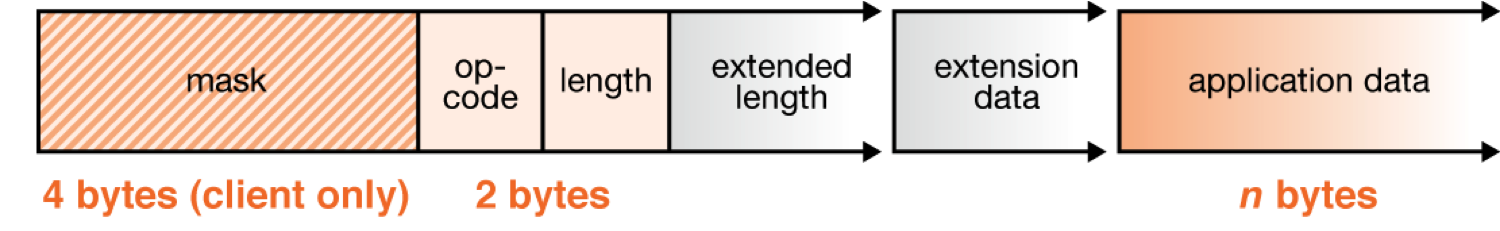
\includegraphics[height=1in,width=7.12in]{./images/websockets/WebSocketFrame.png}  
\caption{\small \sl The Websocket frame \label{fig:websocket_frame}}
\end{figure}

\begin{figure}
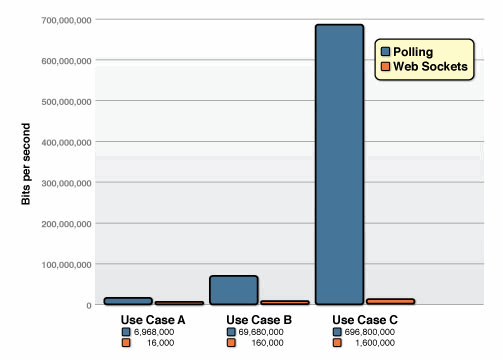
\includegraphics[height=3.5in,width=6.23in]{./images/websockets/poll-ws-compare.png}  
\caption{\small \sl Websocket vs. HTTP Polling
\label{fig:websocket_ws_vs_polling}}
\end{figure}

After some further searching on the web, a forum answer\cite{websockets3} by the
founder of Tavendo, which develops Autobahn - A well-known set of Websocket libraries for
Javascript, Python and Android:\newline

\begin{quotation}
On a LAN, you can get Round-trip times for messages over WebSocket of 200
microsec (from browser JS to WebSocket server and back), which is similar to raw
ICMP pings. On MAN, it's around 10ms, WAN (over residential ADSL to server in
same country) around 30ms, and so on up to around 120-200ms via 3.5G. The point
is: WebSocket does add virtually no latency to the one you will get anyway,
based on the network.\newline

The wire level overhead of WebSocket (compared to raw TCP) is between 2 octets
(unmasked payload of length < 126 octets) and 14 octets (masked payload of
length > 64k) per message (the former numbers assume the message is not
fragmented into multiple WebSocket frames). Very low.\newline

More so: with a WebSocket implementation capable of streaming processing, you
can (after the initial WebSocket handshake), start a single WebSocket message
and frame in each direction and then send up to 2\^63 octets with no overhead at
all. Essentially this renders WebSocket a fancy prelude for raw TCP. Caveat:
intermediaries may fragment the traffic at their own decision. However, if you
run WSS (that is secure WS = TLS), no intermediaries can interfere, and there
you are: raw TCP, with a HTTP compatible prelude (WS handshake).
\end{quotation}

This answer deems Websockets a fast protocol, appropriate for fast-paced games
such as the one described in this paper.\newline

Moreover, Websockets is designed with security standards and easy development in
mind. It has built - in connection management mechanisms that would easily fit
further development of this application. It would be basically eliminating
potential huge amounts of planning and development overhead induced by starting
a proprietary implementation on top of TCP. \newline
